\section{BGP}
\subsection{Forwarding with CIDR}
\begin{itemize}
    \item Longest Prefix Match
\end{itemize}
\begin{figure}[H]
    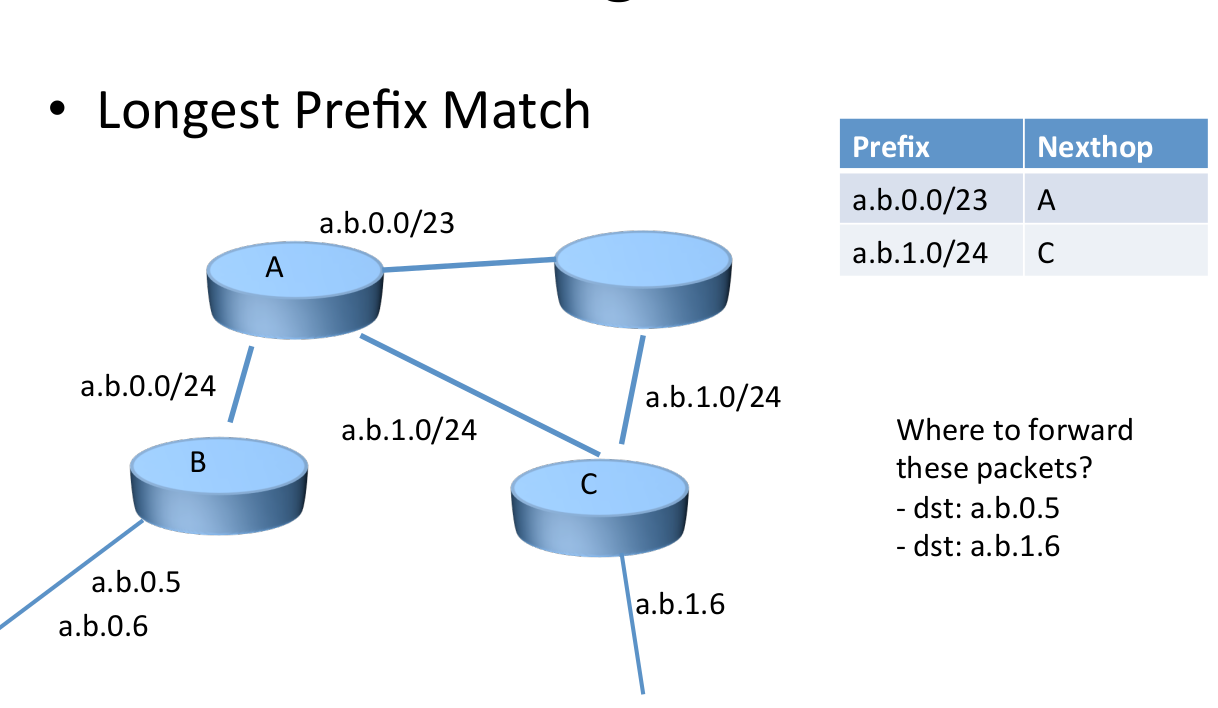
\includegraphics[width=\textwidth]{lazy/longestprefix.png}
\end{figure}

\subsection{Some BGP Challenges}
\begin{itemize}
    \item Convergence
    \item Traffic engineering
          \begin{itemize}
              \item How to assure certain routes are selected
          \end{itemize}
    \item Scaling (route reflectors)
    \item Security
\end{itemize}

\subsection{Convergence}
\begin{itemize}
    \item Given a change, how long until the network re-stabilizes?
          \begin{itemize}
              \item Depends on change: sometimes never
              \item Open research problem: ``tweak and pray''
              \item Distributed setting is challenging
          \end{itemize}
    \item Some reasons for change
          \begin{itemize}
              \item Topology changes
              \item BGP session failures
              \item Changes in policy
              \item Conflicts between policies can cause oscillation
          \end{itemize}
\end{itemize}
\subsection{Routing Change: Before and After}
\begin{figure}[H]
    \tikzsetnextfilename{routing-before-after}
    \begin{tikzpicture}[every node/.style={ellipse, fill=gray!40, minimum height=1cm, minimum width=1.5cm}, node distance=1cm]
        \node (0b) {0};
        \node[below left=of 0b] (1b) {1};
        \node[below right=of 0b] (2b) {2};
        \node[below right=of 1b] (3b) {3};

        \draw[red,->] (1b) -- (0b) node[fill=none,left, pos=0.8] {(1, 0)};
        \draw[red,->] (2b) -- (0b) node[fill=none,right, pos=0.8] {(2, 0)};
        \draw[red,->] (3b) -- (1b) node[fill=none,left, pos=0] {(3, 1, 0)};
        \draw (1b) -- (2b) -- (3b);

        \node[right=4cm of 0b] (0a) {0};
        \node[below left=of 0a] (1a) {1};
        \node[below right=of 0a] (2a) {2};
        \node[below right=of 1a] (3a) {3};

        \draw (0a) -- (1a) -- (3a);
        \path (0a) -- (1a) node[pos=0.5, draw,red,starburst,fill=orange,minimum height=2cm,minimum width=3cm, line width=1.5pt,scale=0.25] {};

        \draw[red,->] (1a) -- (2a) node[fill=none,above,pos=0.6] {(1, 2, 0)};
        \draw[red,->] (3a) -- (2a) node[fill=none,right,pos=0] {(3, 2, 0)};
        \draw[red,->] (2a) -- (0a) node[fill=none,right,pos=0.8] {(2, 0)};
    \end{tikzpicture}
\end{figure}
\subsection{Routing Change: Path Exploration}
\begin{itemize}
    \item AS 1
          \begin{itemize}
              \item Delete the route (1, 0)
              \item Switch to next route (1, 2, 0)
              \item Send route (1, 2, 0) to AS 3
          \end{itemize}
    \item AS 3
          \begin{itemize}
              \item Sees (1, 2, 0) replace (1, 0)
              \item Compares to route (2, 0)
              \item Switches to using AS 2
          \end{itemize}
\end{itemize}
\begin{figure}[H]
    \tikzsetnextfilename{routing-path-exploration}
    \begin{tikzpicture}[every node/.style={ellipse, fill=gray!40, minimum height=1cm, minimum width=1.5cm}, node distance=1cm]
        \node (0a) {0};
        \node[below left=of 0a] (1a) {1};
        \node[below right=of 0a] (2a) {2};
        \node[below right=of 1a] (3a) {3};

        \draw (0a) -- (1a) -- (3a);
        \path (0a) -- (1a) node[pos=0.5, draw,red,starburst,fill=orange,minimum height=2cm,minimum width=3cm, line width=1.5pt,scale=0.25] {};

        \draw[red,->] (1a) -- (2a) node[fill=none,above,pos=0.6] {(1, 2, 0)};
        \draw[red,->] (3a) -- (2a) node[fill=none,right,pos=0] {(3, 2, 0)};
        \draw[red,->] (2a) -- (0a) node[fill=none,right,pos=0.8] {(2, 0)};
    \end{tikzpicture}
\end{figure}
\begin{itemize}
    \item Initial Situation
          \begin{itemize}
              \item Destination 0 is alive
              \item All ASes use direct path
          \end{itemize}
    \item When destination dies
          \begin{itemize}
              \item All ASes lose direct path
              \item All switch to longer paths
              \item Eventually withdrawn
          \end{itemize}
    \item e.g. AS 2
          \begin{itemize}
              \item (2, 0) $\rightarrow$ (2, 1, 0)
              \item (2, 1, 0) $\rightarrow$ (2, 3, 0)
              \item (2, 3, 0) $\rightarrow$ (2, 1, 3, 0)
              \item (2, 1, 3, 0) $\rightarrow$ \Null
          \end{itemize}
    \item \emph{Convergence may be slow!}
\end{itemize}
\begin{figure}[H]
    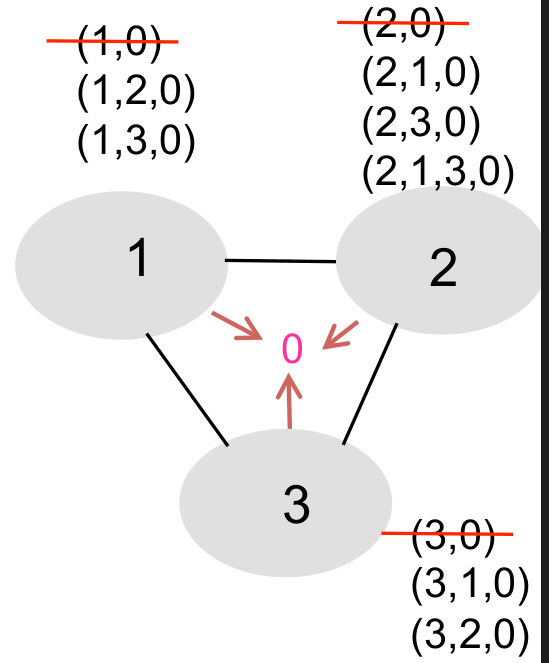
\includegraphics[scale=0.25]{lazy/routingpathexploration2.png}
\end{figure}

\subsection{Unstable Configurations}
\begin{itemize}
    \item Due to policy conflicts
\end{itemize}
\begin{figure}[H]
    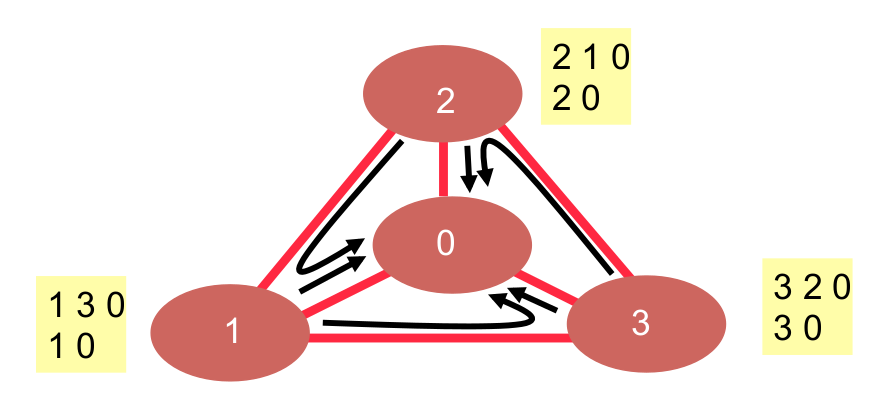
\includegraphics[scale=0.25]{lazy/unstableconfigurations.png}
\end{figure}

\subsection{BGP Security Goals}
\begin{itemize}
    \item Confidential messages exchange between neighbors
    \item \emph{Validity of routing information}
          \begin{itemize}
              \item Origin, Path, Policy
          \end{itemize}
    \item Correspondence to the data path
\end{itemize}

\subsection{Origin: IP Address Ownership and Hijacking}
\begin{itemize}
    \item IP address block assignment
          \begin{itemize}
              \item Regional Internet Registries (ARIN, RIPE, APNIC)
              \item Internet Service Providers
          \end{itemize}
    \item Proper Origination of a prefix into BGP
          \begin{itemize}
              \item By the AS who owns the prefix
              \item \dots or, by its upstream provider(s) on its behalf
          \end{itemize}
    \item However, what's to stop someone else?
          \begin{itemize}
              \item Prefix hijacking: another AS originates the prefix
              \item BGP does not verify that the AS is authorized
              \item Registries of prefix ownership are inaccurate
          \end{itemize}
\end{itemize}

\subsection{Prefix Hijacking}
\begin{figure}[H]
    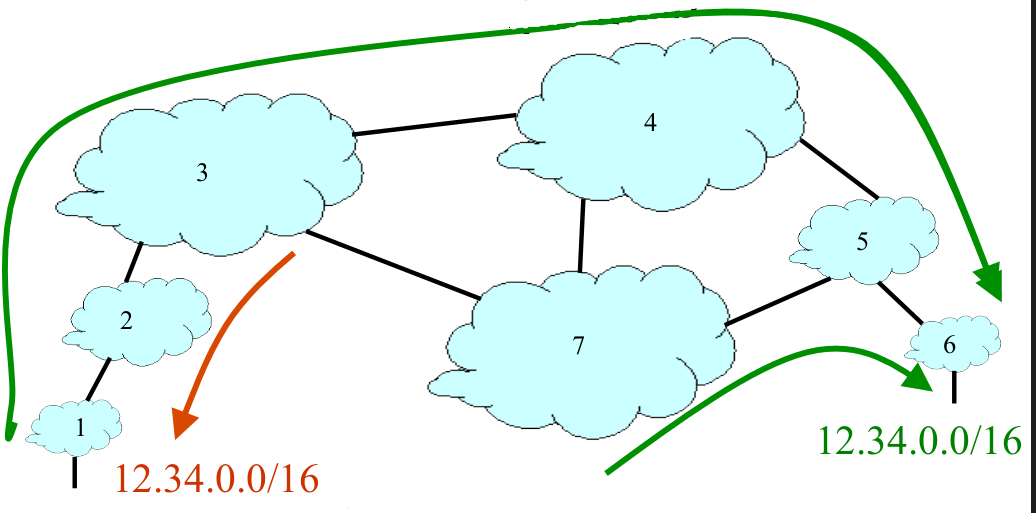
\includegraphics[scale=0.5]{lazy/prefixhijacking.png}
\end{figure}
\begin{itemize}
    \item Consequences for the affected ASes
          \begin{itemize}
              \item Blackhole: data traffic is discarded
              \item Snooping: data traffic is inspected and then redirected
              \item Impersonation: data traffic is sent to bogus destinations
          \end{itemize}
\end{itemize}

\subsection{Hijacking is Hard to Debug}
\begin{itemize}
    \item Real origin AS doesn't see the problem
          \begin{itemize}
              \item Picks its own route
              \item Might not even learn the bogus route
          \end{itemize}
    \item May not cause loss of connectivity
          \begin{itemize}
              \item e.g. if the bogus AS snoops and redirects
              \item \dots may only cause performance degradation
          \end{itemize}
    \item Or, loss of connectivity is isolated
          \begin{itemize}
              \item e.g. only for sources in parts of the internet
          \end{itemize}
    \item Diagnosing prefix hijacking
          \begin{itemize}
              \item Analyzing updates from many vantage points
              \item Launching traceroute from many vantage points
          \end{itemize}
\end{itemize}

\subsection{Sub-Prefix Hijacking}
\begin{figure}[H]
    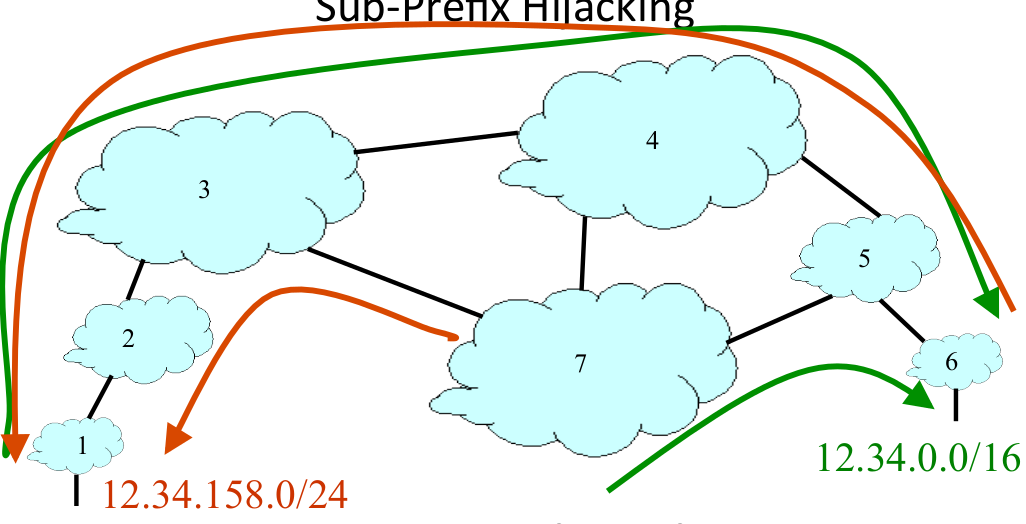
\includegraphics[scale=0.5]{lazy/subprefixhijacking.png}
\end{figure}
\begin{itemize}
    \item Originating in a more-specific prefix
          \begin{itemize}
              \item Every AS picks the bogus route for that prefix
              \item Traffic follows the longest matching prefix
          \end{itemize}
\end{itemize}

\subsection{How to Hijack a Prefix}
\begin{itemize}
    \item The hijacking AS has
          \begin{itemize}
              \item Router with eBGP sessions(s)
              \item Configured to originate the prefix
          \end{itemize}
    \item Getting access to the router
          \begin{itemize}
              \item Network operator makes configuration mistake
              \item Disgruntled operator launches an attack
              \item Outsider breaks in to the router and reconfigures
          \end{itemize}
    \item Getting other ASes to believe bogus route
          \begin{itemize}
              \item Neighbor ASes not filtering the routes
              \item e.g. by allowing only expected prefixes
              \item But, specifying filters on \emph{peering} links is hard
          \end{itemize}
\end{itemize}

\subsection{Pakistan YouTube Incident}
\begin{itemize}
    \item YouTube has prefix 208/65/152.0/22
    \item Pakistan's government order YouTube blocked
    \item Pakistan Telecom (AS 17557) announces 208.65.153.0/24 in the wrong direction (outwards!)
    \item Longest prefix match caused worldwide outage
    \item \url{https://www.youtube.com/watch?v=IzLPKuAOe50}
\end{itemize}

\subsection{Many other incidents}
\begin{itemize}
    \item Spammers steal unused IP space to hide
          \begin{itemize}
              \item Announce very short prefixes (e.g. /8). Why?
              \item For a short amount of time
          \end{itemize}
    \item China incident, April 8, 2010
          \begin{itemize}
              \item China's Telecom AS23724 generally announces 40 prefixes
              \item On April 8, announced $\approx$ 37,000 prefixes
              \item About 10\% leaked outside of China
              \item Suddenly, going to \url{www.dell.com} might have you routing through AS23724!
          \end{itemize}
\end{itemize}

\subsection{Attacks on BGP Paths}
\begin{itemize}
    \item Remove an AS from the path
          \begin{itemize}
              \item e.g. 701 3715 88 $\to$ 701 88
          \end{itemize}
    \item Why?
          \begin{itemize}
              \item Attract sources that would normally avoid AS 3715
              \item Make AS 88 look like it is closer to the core
              \item Can fool loop detection!
          \end{itemize}
    \item May be hard to tell whether this is a lie
          \begin{itemize}
              \item 88 could indeed connect directly to 701!
          \end{itemize}
\end{itemize}

\begin{itemize}
    \item Adding ASes to the path
          \begin{itemize}
              \item e.g. 701 88 $\to$ 701 3715 88
          \end{itemize}
    \item Why?
          \begin{itemize}
              \item Trigger lookup detection in AS 3715
                    \begin{itemize}
                        \item This would block unwanted traffic from AS 3715!
                    \end{itemize}
              \item Make your AS look more connected
          \end{itemize}
    \item Who can tell this is a lie?
          \begin{itemize}
              \item AS 3715 could, if it could see the route
              \item AS 88 could, but would it really care?
          \end{itemize}
\end{itemize}


\begin{itemize}
    \item Adding ASes at the end of the path
          \begin{itemize}
              \item e.g. 701 88 $\to$ 701 88 3
          \end{itemize}
    \item Why?
          \begin{itemize}
              \item Evade detection for a bogus route (if added AS is legitimate owner of a prefix)
          \end{itemize}
    \item Hard to tell that the path is bogus!
\end{itemize}